%!TEX root = ../thesis.tex

\chapter{Theory}
This chapter describe background theory about parallelism, why it has become a highly relevant topic in modern system architectures. It also describes the different frameworks and libraries evaluated in this work, as well as some typical parallelizable problems. Finally, some suitable benchmarking algorithms are presented and a motivation why each algorithm is suitable for this kind of evaluation.

\section{The rise of parallelism} 
As mentioned in section \ref{sec:IntroductionMotivation}, the performance inclination of single-cored CPU's has reached a limit. The reason for this decline is due to three walls.

The \textbf{ILP-wall} which states that there is not enough instruction level parallelism to keep the CPU busy. Some techniques do however exist such as Very Large Instruction Word (VLIW) and the Superscalar Architecture but are limited by the hardware complexity.

The second wall, the \textbf{Memory wall} is reached because of the gap between the CPU speed and accesses to off-chip memory.

As mentioned in section \ref{sec:IntroductionMotivation} and visualized in figure \ref{fig:CPUstats}, Moore's law is still valid, but the increased amount of on-chip micro transistors needs an increased amount of power, this leads to overheating problems and has been named the \textbf{Power wall}.

The solution to all of these problems are however the same, it is not possible to increase the single-thread performance, but we can put more cores on a chip. Today, all major CPU manufacturers develop multi-core CPU's, and most devices used in our everyday life such as smartphones, laptops 
and desktop CPU's have a multi-core architecture, and the number of cores on a chip seems to be increasing, see figure \ref{fig:CPUstats}

\begin{figure}[!h]
    \centering
    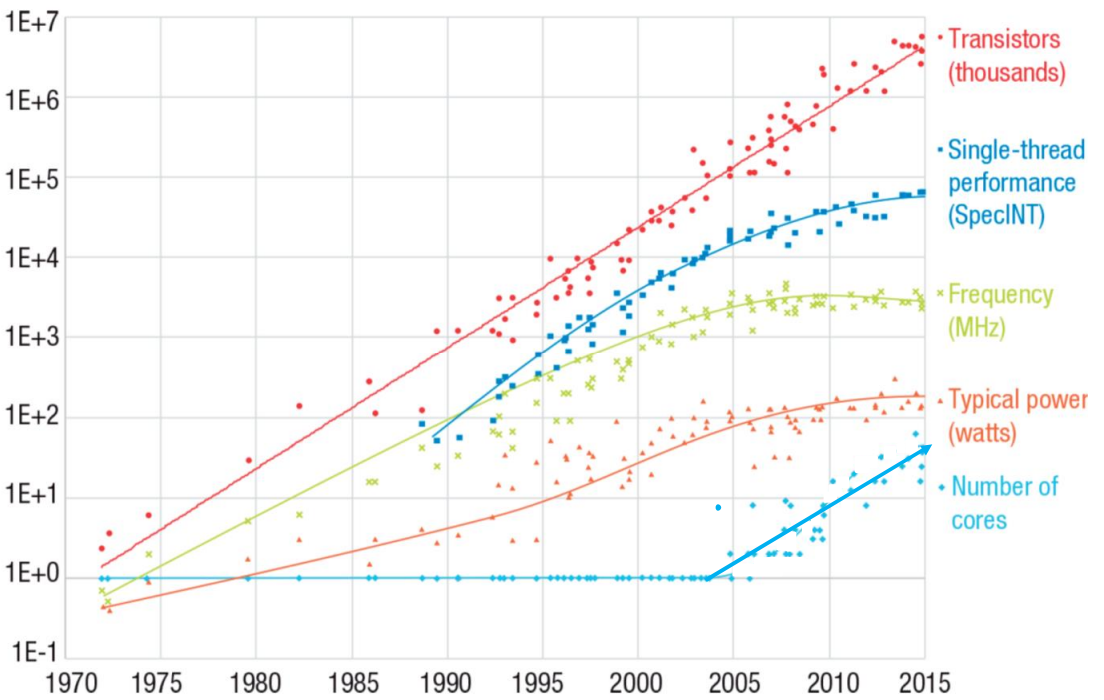
\includegraphics[width=0.8\textwidth]{Introduction/Figs/CPUStats.png}
    \caption{Statistics of development for CPU's. \cite{CPUStats}}
    \label{fig:CPUstats}
\end{figure}

The idea of putting multiple cores on a single chip which may be run in parallel is not new technology, GPU's has long been using this architecture and modern GPU chips contains hundreds of cores. This massive amount of parallelism and parallel computing power are designed to render graphics on screen and perform fast algebraic calculations such as matrix or vector additions, and is thus parallel in nature. But it can also be used for more general purpose computing, as quoted by Thompson et. al. "...Most of this time, however, this power is going unused because it is only
being exploited by graphics applications" \cite{thompson2002gpgpu}.


\subsection{History}
With the release of programmable shaders and floating point precision GPUs in 2001, the idea of performing general purpose computing on the GPU was born. Early research on the subject implemented simple, well-parallelizable problems such as vector or matrix additions, and one of the first scientific GPGPU problems that outperformed the CPU was a implementation of LU factorization. \cite{CUDAtoOpenCL}. Another research on the subject performed by Thompson et. al. from 2002 showed that a simple arithmetic operation applied to all elements of a vector of varying sized, outperformed the CPU once the problem size grew large enough which is generally the case for GPGPU.\cite{thompson2002gpgpu}.

These early adaptations of GPGPU used the traditional rendering pipeline by performing computations in the shaders of the application, using the two major application programming interfaces (API) OpenGL and DirectX. Although this approach adds some limitations, it is still quite widespread and are still in use today. Since then, both OpenGL and DirectX has released shaders specifically purposed for GPGPU. These types of shaders are known as Compute Shaders (CS), and Microsoft released their CS support with the DirectCompute as a part of the DirectX collection of APIs.

Later on Nvidia realized the potential of GPGPU and developed the CUDA framework to make GPGPU programming easier by adding lots of features and simplyfing the data transfer. Later on, OpenCL was released with the same purpose, and a lot of backing major companies such as Apple and IBM. It is today maintained by the Khronos group, which also maintains OpenGL.



\section{Frameworks}
This section briefly describes the different frameworks and APIs that are a subject of comparison in this comparative study. The popularity of the frameworks is based upon the chart in figure \ref{fig:GoogleTrendsPopularity} from Google Trends.

\subsection{CUDA}
Released in 2007, CUDA developed by Nvidia was the first major GPGPU framework to be released. It aims to make the parallelization of a problem more manageable by providing a easy to work with API. One downside of CUDA is that is has a weak portability and can only be run on Nvidia GPU's. Despite this limitation it is a very popular framework among GPGPU developers, see figure \ref{fig:GoogleTrendsPopularity}. \cite{AboutCuda} 

\subsection{OpenCL}
For a couple of years, CUDA was the only framework developed for the sole purpose of GPGPU and Nvidia had no competitors on the GPGPU front. That is until Apple took the initiative to develop a competitor, and backed by a lot of major companies, OpenCL was developed. OpenCL sought to offer a more portable and wide variety of parallel devices, and OpenCL offers the ability to run parallel implementations on other devices than just GPUs such as FPGA and ARM devices. It is an open standard, much like OpenGL and OpenCL implementations are available from Apple, AMD, Intel, Nvidia and more. \cite{KhronosOpenCL}



\subsection{DirectCompute}
Initially released with the DirectX 11 API, DirectCompute is Microsoft's technology for GPGPU, and unlike CUDA or OpenCL which relies on launching kernels, DirectCompute runs a CS as a part of the graphics pipeline. Although released with the DirectX 11 API, DirectCompute runs on GPUs that use either DirectX 10 or 11. \cite{NVidiaDirectCompute} 

\subsection{SkePU 2}
SkePU is a high-level skeleton programming framework originally developed by Johan Enmyren and Christoph W. Kessler at Linköping University \cite{enmyren2010skepu}. The framework aims to simplify the parallelization of a implementation by using skeleton functions such as map and reduce which are common parallel algorithms, which makes SkePU very different from the previously mentioned frameworks. When using SkePU, the developer specifies what backend the implementation should run on and the currently available backends are sequential C, OpenMP, OpenCL, CUDA, and multi-GPU OpenCL and CUDA \cite{LiUSkePU}. The major revision SkePU 2 was designed by August Ernstsson, Lu Li and Christoph Kessler and is today maintained by August Ernstsson. Further mentions of SkePU will refer to SkePU 2.


\begin{figure}[!htbp]
    \centering
    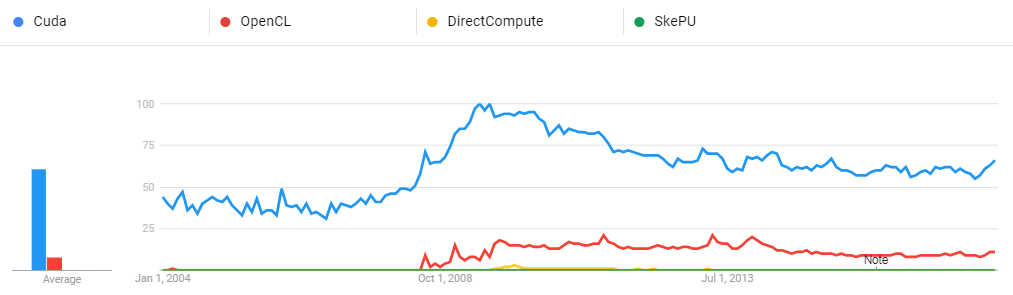
\includegraphics[width=\textwidth]{Theory/Figs/GoogleTrendsComparison.png}
    \caption{Popularity over time of CUDA, OpenCL and DirectCompute. Numbers represent search interest relative to the highest point on the chart for the given region and time. \ \textbf{Source:} Google trends}
    \label{fig:GoogleTrendsPopularity}
\end{figure}





\section{Algorithm}

\subsection{N-Body}

\subsection{Parallel QuickSort}

\subsection{Distance transform}

\subsection{Choice of algorithm}




%--------------------------------------------------------%
%----------------------Nomenclature----------------------%
%--------------------------------------------------------%

\nomenclature[z-VLIW]{VLIW}{Very Large Instruction Word}
\nomenclature[z-CS]{CS}{Compute Shader}
\nomenclature[z-API]{API}{Application Programming Interface}